% ********************************************************************
% *                  Format for IMVIP 2019  papers,                  *
% *         based on the IMVIP 2001, 2006, 2014-2018 templates       *
% ********************************************************************
\documentclass[a4paper,11pt]{article}



\setlength{\topmargin}{-0.5cm}
\setlength{\headsep}{.5cm}
%\setlength{\footskip}{1.0cm}
\setlength{\textheight}{24cm}
\setlength{\textwidth}{17cm}
\setlength{\evensidemargin}{-.5cm}
\setlength{\oddsidemargin}{-.5cm}



\usepackage{fourier}
\usepackage{color}
\usepackage{graphicx}
\usepackage{url}
\usepackage[affil-it]{authblk}
\usepackage{amsmath}
\usepackage{wrapfig}
\usepackage{xspace}
\usepackage{hyperref}
\usepackage[T1]{fontenc}
\usepackage{times}


\pagestyle{empty}

%%%%
\begin{document}

\title{Author Instructions for IMVIP 2019}

\author{Tomás Pettit}
\affil{Anonymous Affiliation}
\date{}
\maketitle
\thispagestyle{empty}

\begin{abstract}
This study explores the development of a deep learning system to classify 10 different categories of waste. Recognizing waste from images is a challenging task because many types appear very similar, and the presentation of waste can vary significantly. This research compares two main methods: a custom-built Convolutional Neural Network (CNN) and a Transfer Learning approach that utilizes a pre-trained model as its basis, leveraging a comprehensive garbage dataset.
\end{abstract}
\textbf{Keywords:} Image Classification, Convolutional Neural Networks, Transfer Learning, MobileNetV2.


\section{Introduction}
The dataset is derived from the Garbage Dataset (GD)~\cite{kunwar2026}, a publicly available benchmark for automated waste segregation. The images were collected through multiple methods including a mobile application and curated web sources, and exhibit realistic variability in lighting, background, and object occlusion — which makes the classification task genuinely challenging.

\section{Data and Pre-Processing}
The first thing I did was to initialise any of the variables I will be using that will detail how I will be processing my data. The seed that I set is \texttt{RANDOM\_SEED = 419414} for my student number, this will allow for reproducibility of my results. I then have the batch sizes for my data in batches of \texttt{BATCH\_SIZE=32}, dealing with image sizes of \texttt{IMAGE\_SIZE=[(64$\times$64),(128$\times$128),(224$\times$224)]}, and a number of epochs \texttt{EPOCH=[3,10,15]}. Computational tasks were performed locally using T4 GPU, which is faster than CPU.

\subsection{Dataset Description}
The image dataset being used is a subset of the Garbage dataset containing 10 folders named after the type of waste contained in its images. The images in use are $512\times512$ but will be rescaled to $128\times128$ and $64\times64$, grayscaled and/or augmented to explore different hyperparameters and compare models.

\subsection{Exploratory Analysis}
The dataset comprises \textbf{12,259 JPEG images} totalling approximately $\sim$400~MB across \textbf{10 waste categories}. Figure~\ref{fig:class_dist} visualises the distribution.

\begin{figure}[ht]
    \centering
    
\includegraphics[width=0.75\linewidth]{images/class_distribution.png}
    \caption{Class distribution of the cleaned dataset}
    \label{fig:class_dist}
\end{figure}

\subsection{Preprocessing and Splits}
The dataset comprises images with three colour channels (RGB). As these involve values ranging from 0 to 255, it was essential to normalise the training data to facilitate data flow between layers and prevent vanishing or exploding gradients. The data was partitioned into three distinct sets to ensure a robust training and evaluation process:
\begin{itemize}
    \item 70\% training (8,581 images) and 30\% temporary were created first;
    \item the temporary set was then divided into 10\% validation (1,226 images)
    \item 20\% test (2,452 images).
\end{itemize}


\section{Experiments}
\subsection{CNN Experiments from Scratch}
Seven custom CNN variants were trained to identify the best architecture and preprocessing strategy before applying transfer learning. All share a 3-layer backbone ($3\times3$ convolutions, filter counts 32/64/128, $2\times2$ max-pooling, 128-unit dense head) and use Adam~\cite{kingma2017adam} with sparse categorical cross-entropy (batch size 32). Each experiment varied one factor at a time; results are summarised in Table~\ref{tab:cnn_scratch}.
 
\begin{table}[ht]
    \centering
    \begin{tabular}{|l|c|c|c|c|}
    \hline
    \textbf{Model} & \textbf{Input} & \textbf{Ep.}
      & \textbf{Train (\%)} & \textbf{Val (\%)} \\ \hline
    Baseline                   & 128$\times$128 RGB  & 10 & 95.3  & 62.5  \\ \hline
    + Dropout (0.2)            & 128$\times$128 RGB  & 10 & 96.3  & 64.4  \\ \hline
    Baseline (64$\times$64)    & 64$\times$64 RGB    & 10 & 89.1  & $\sim$62 \\ \hline
    + Aug (aggressive)         & 128$\times$128 RGB  & 10 & $>$15.0 & 16.1 \\ \hline
    \textbf{+ Aug (mild)}      & \textbf{64$\times$64 RGB} & \textbf{15} & \textbf{81.8} & \textbf{70.2} \\ \hline
    + Deeper (256 filters)     & 64$\times$64 RGB    & 15 & $\sim$81.5 & 67.9 \\ \hline
    + Deeper (128 filters)     & 64$\times$64 RGB    & 15 & $\sim$73.5 & $>$64 \\ \hline
    Grayscale (mild aug)       & 64$\times$64 Gray   & 15 & 73.9  & 61.6  \\ \hline
    \end{tabular}
    \caption{Custom CNN ablation results. Bold = best scratch configuration.}
    \label{tab:cnn_scratch}
\end{table}
 
Three key findings emerge. First, \textbf{regularisation helps but is insufficient alone}: dropout raised validation accuracy from 62.5\% to 66.3\%, yet the train--val gap remained large, indicating persistent overfitting from the dataset size rather than model capacity. Second, \textbf{augmentation quality is critical}: aggressive augmentation (vertical flip, 0.3 rotation, zoom, brightness, contrast) destroyed performance (52.6\%), while mild augmentation (horizontal flip + 0.05 rotation) on 64$\times$64 images achieved the best scratch result at \textbf{70.3\%} validation accuracy with a reduced train--val gap of 0.15. Third, \textbf{colour is essential}: removing colour information dropped accuracy by 10.8 points (70.3\% $\to$ 59.5\%), confirming that hue is a key discriminating cue for categories such as glass vs.\ plastic and biological waste vs.\ cardboard. Adding depth (a fourth conv block at 256 or 128 filters) failed to improve on the 3-layer design, confirming that the dataset is too small to benefit from extra capacity.

\subsection{Transfer Learning Analysis - MobileNetV2}
\subsubsection{Motivation and Setup}
The best custom CNN is constrained by dataset size: with $\sim$8,600 training images, a scratch model cannot learn the richness of features available from millions of diverse images. Transfer learning~\cite{pan2009survey} addresses this by initialising with MobileNetV2 weights pre-trained on ImageNet, which provide well-calibrated low-level and mid-level visual representations that generalise to new domains.
 
Images were resized to $224\times224$ to match the MobileNetV2 input requirement. The MobileNetV2 \textit{preprocess\_input} function was applied inline as a Keras Lambda layer. A Global Average Pooling layer, a 128-unit Dense layer (ReLU, Dropout 0.3), and a 10-way softmax output were appended as the classification head.
 
\subsubsection{Three Transfer Learning Runs}
\begin{itemize}
    \item \textbf{Initial Fine-tuning Attempt}: the top 30 MobileNetV2 layers were unfrozen immediately and trained at a low learning rate ($\alpha = 10^{-5}$) for 10 epochs (\texttt{EPOCH[1]=10}) without first establishing a frozen baseline. This achieved \textbf{85.6\%} validation accuracy, a major improvement over the best custom CNN but suboptimal, as the pre-trained features were adapted from the start.
 
    \item \textbf{Frozen Base (RERUN)}: following the recommended two-stage workflow, all MobileNetV2 base layers were frozen and only the newly added classification head was trained (Adam, $\alpha = 10^{-3}$, 10 epochs). This achieved \textbf{91.7\%} validation accuracy — 6.1 points above the initial fine-tuning attempt and 21.4 points above the best custom CNN. Freezing the base forces the model to learn task-specific classification without disrupting the well-tuned ImageNet feature extractor.
 
    \item \textbf{Fine-tuning RERUN}: the top 30 MobileNetV2 layers were unfrozen from the frozen baseline and retrained at $\alpha = 10^{-5}$ for 3 epochs. Validation accuracy matched the frozen baseline at \textbf{91.7\%} without further improvement,
    while adding training complexity and catastrophic forgetting risk. The frozen base model was therefore selected as the final model.
\end{itemize}

\section{Results and Comparison}
\subsection{Model Comparison Summary}
Table~\ref{tab:results} summarises training and validation accuracy across all experiments.
 
\begin{table}[ht]
    \centering
    \begin{tabular}{|l|c|c|c|c|}
    \hline
    \textbf{Model} & \textbf{Input} & \textbf{Ep.}
      & \textbf{Train (\%)} & \textbf{Val (\%)} \\ \hline
    Baseline CNN                     & 128$\times$128 RGB  & 10 & $\sim$95.3 & 62.5 \\ \hline
    CNN + Dropout (0.2)              & 128$\times$128 RGB  & 10 & $\sim$96.3 & $\sim$64.4 \\ \hline
    Baseline CNN (64$\times$64)      & 64$\times$64 RGB    & 10 & $\sim$89.1 & $\sim$62.5 \\ \hline
    CNN + Aug (worst)                & 128$\times$128 RGB  & 10 & $\sim$15   & $\sim$16.1 \\ \hline
    CNN + Aug (best)                 & 64$\times$64 RGB    & 15 & $\sim$81.8 & $>$70.2 \\ \hline
    CNN + Deeper (256 filters)       & 64$\times$64 RGB    & 15 & $\sim$81.5 & $\sim$67.9 \\ \hline
    CNN + Deeper (128 filters)       & 64$\times$64 RGB    & 15 & $\sim$73.5 & $\sim$64 \\ \hline
    CNN + Grayscale                  & 64$\times$64 Gray   & 15 & $\sim$73.8 & $\sim$61.6 \\ \hline
    MobileNetV2 (fine-tuned, init.)  & 224$\times$224 RGB  & 10 & $\sim$96.8 & $>$90.3 \\ \hline
    MobileNetV2 (frozen)             & 224$\times$224 RGB  & 10 & $>$98      & $>$92 \\ \hline
    \textbf{MobileNetV2 (fine-tuned, RERUN)} & \textbf{224$\times$224 RGB} & \textbf{3} & \textbf{$\sim$95.2} & \textbf{$\sim$91.8} \\ \hline
    \end{tabular}
    \caption{Training and validation accuracy across all CNN and transfer learning experiments. Bold row indicates the best model in each category.}
    \label{tab:results}
\end{table}


\subsection{Final Test Set Evaluation}
The fine-tune RERUN MobileNetV2 model was evaluated on the held-out test set (20\% of data, never seen during training or validation), achieving \textbf{93\% test accuracy} with a strong macro-averaged F1 score of \textbf{0.92}.

\subsection{Per-Class Performance}
 
Figure~\ref{fig:confusion_matrix} shows the confusion matrix on the test set.
\begin{figure}[ht]
    \centering
    
\includegraphics[width=0.7\linewidth]{images/confusion_matrix.png}
    \caption{Confusion matrix for the fine-tune RERUN MobileNetV2 model on the held-out test set. Off-diagonal concentrations reveal the most frequent misclassification pairs.}
    \label{fig:confusion_matrix}
\end{figure}

The model performs well on visually distinctive classes (clothes, shoes, biological waste), but confuses visually similar materials. The three principal failure pairs are:
 
\begin{itemize}
    \item \textbf{Glass $\leftrightarrow$ Plastic}: both classes include transparent or semi-transparent bottles with similar geometry.
    \item \textbf{Paper $\leftrightarrow$ Cardboard}: shared flat texture and brown hue make these the hardest pair to separate.
    \item \textbf{Trash $\leftrightarrow$ Metal}: the \textit{Trash} class has the lowest per-class F1 (0.87 for plastic, lower for trash) due to its heterogeneous, multi-material appearance.
\end{itemize}
 
\textit{Trash} is the smallest class at only 453 images — contributes to its weaker recall.

\section{Real-World Test}
To assess practical generalisation beyond the held-out test set, the final frozen MobileNetV2 model was evaluated on four personal photographs taken with a smartphone camera (battery, cardboard, glass, plastic). Both RGB and grayscale inference were compared. Figure~\ref{fig:rw_rgb} shows the RGB predictions and Figure~\ref{fig:rw_gray} the grayscale predictions.

\begin{figure}[ht]
    \centering
    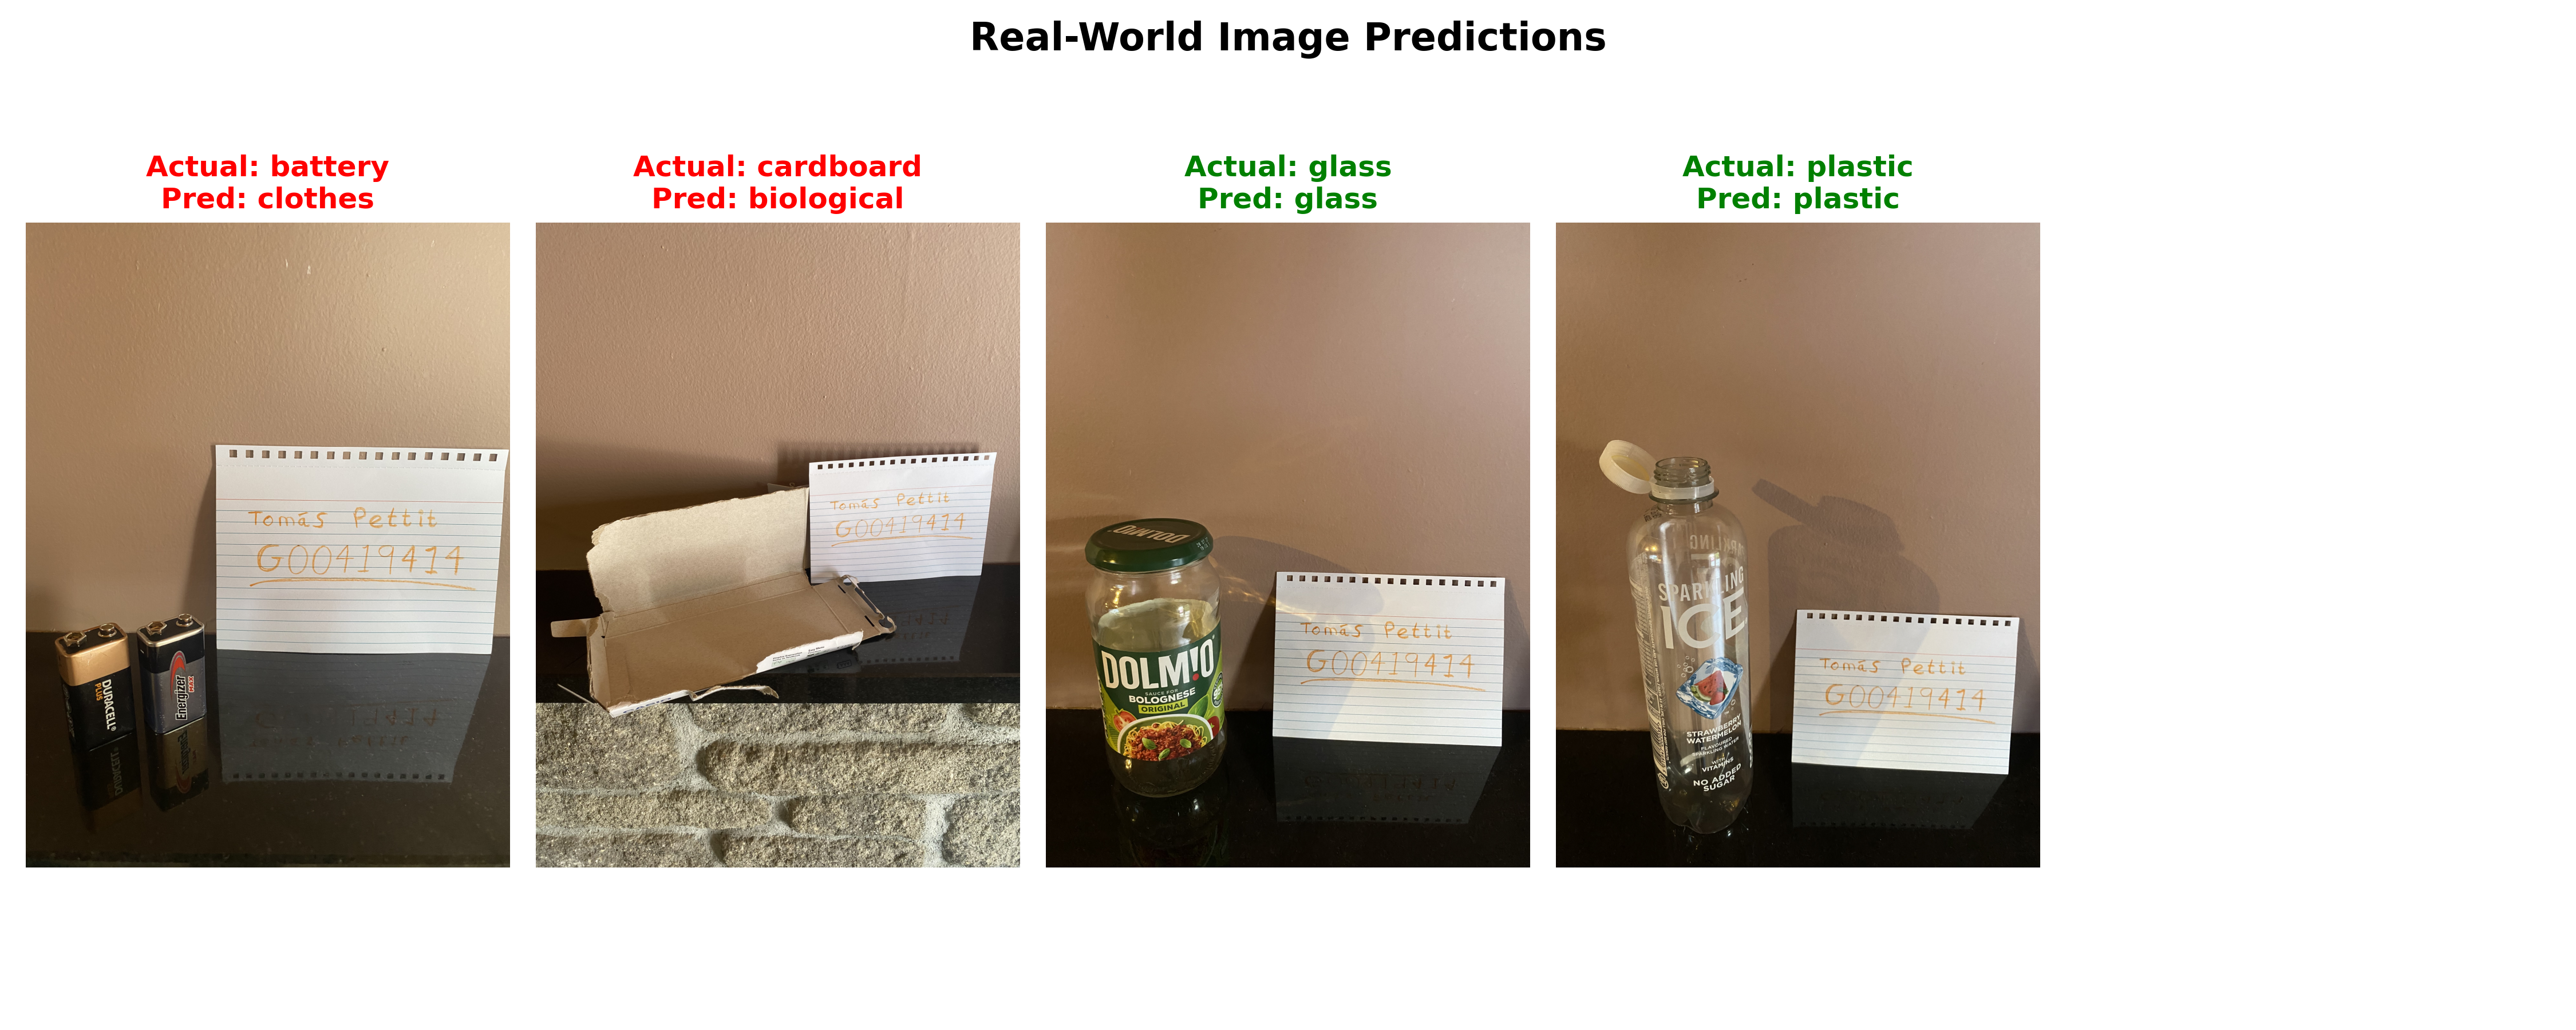
\includegraphics[width=0.65\linewidth]{images/sample_predictions.png}
    \caption{Real-world RGB image predictions. Titles are green (correct) or red (incorrect).}
    \label{fig:rw_rgb}
\end{figure}

\begin{figure}
    \centering
    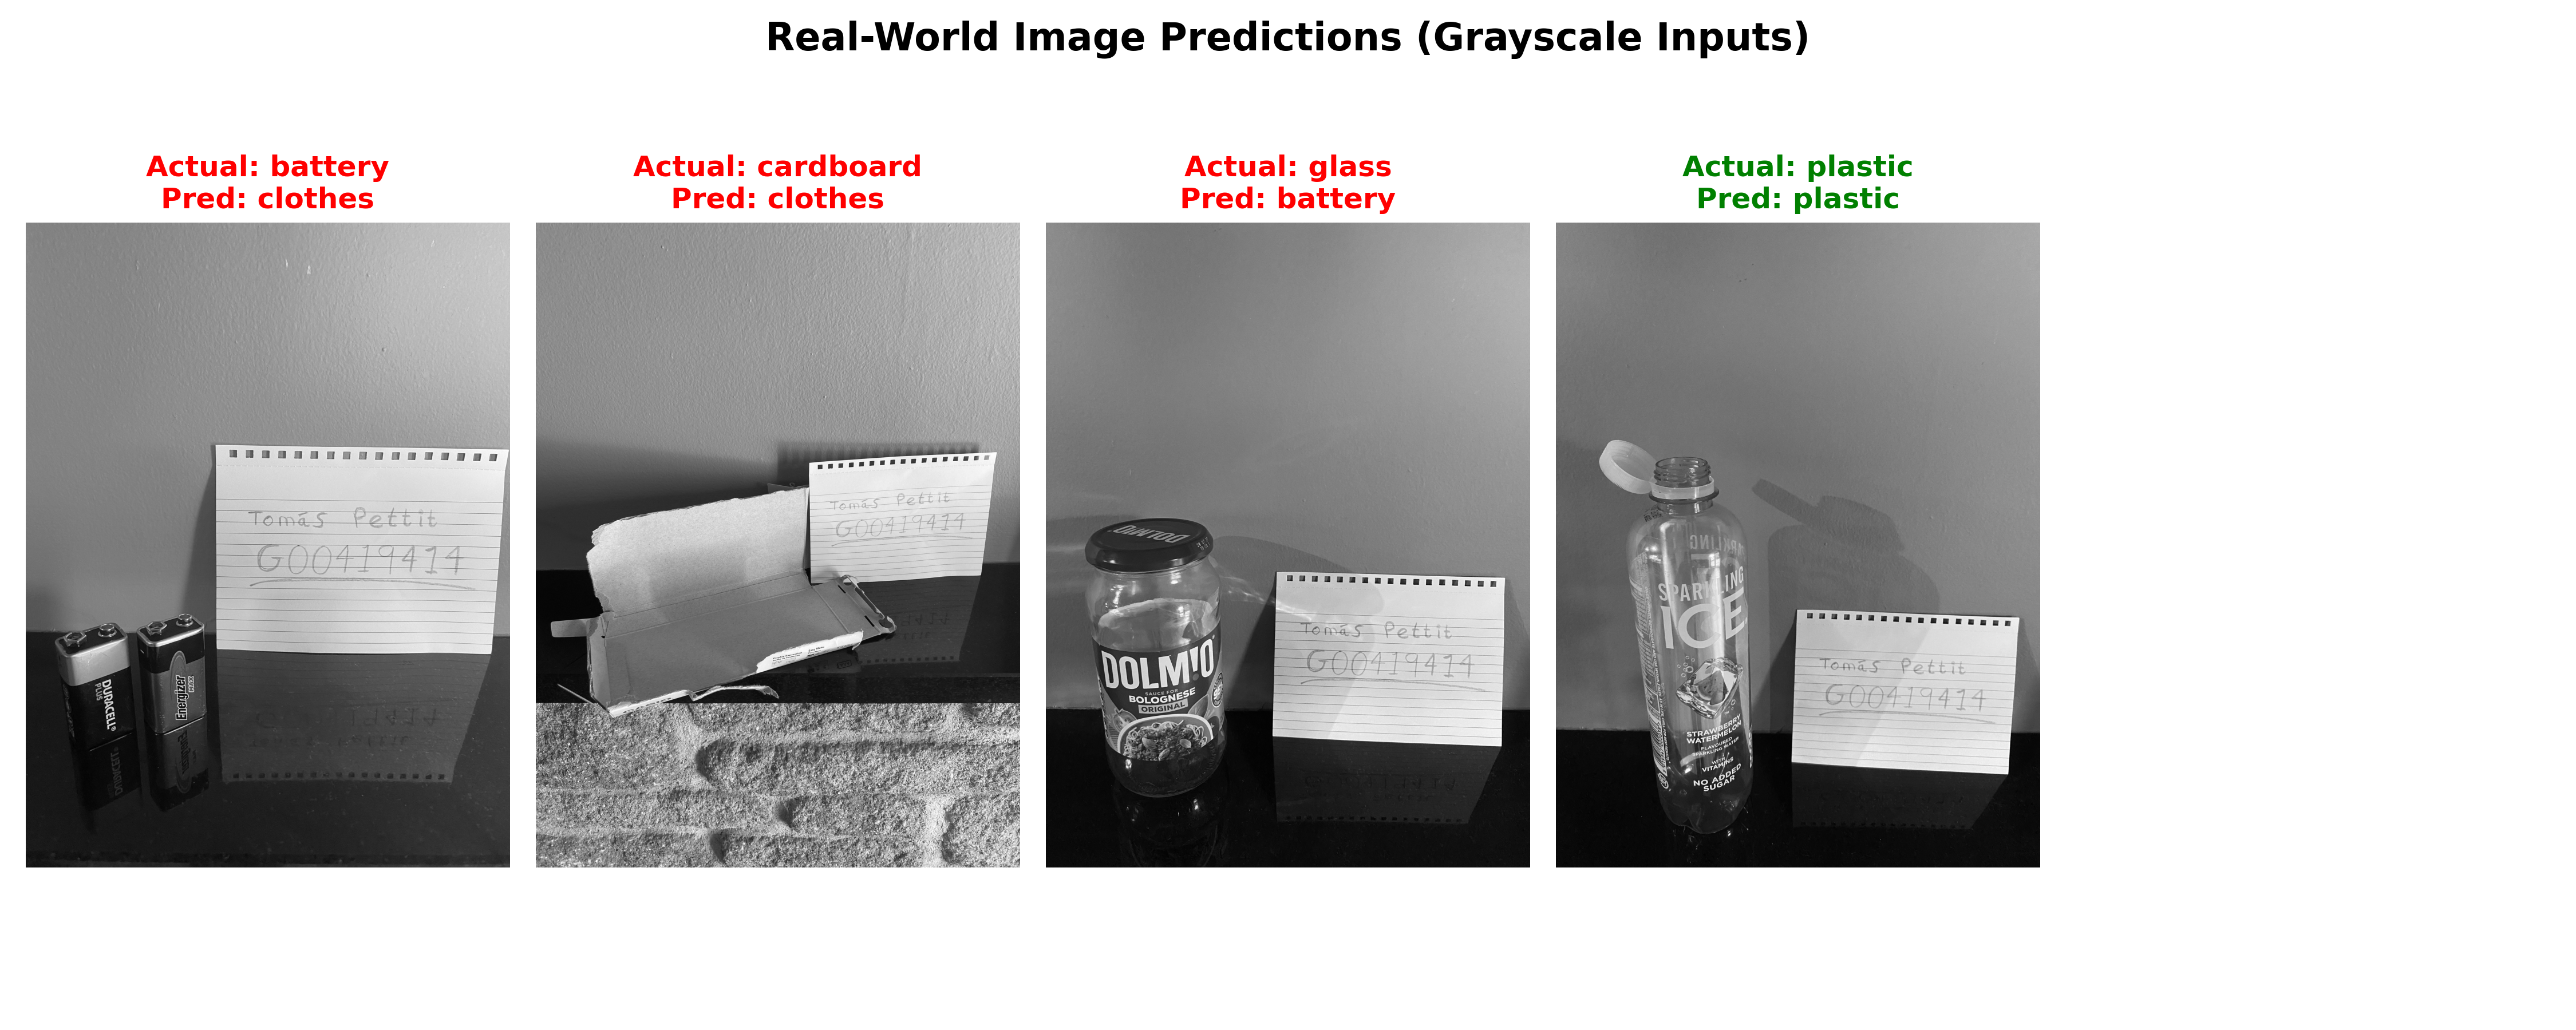
\includegraphics[width=0.65\linewidth]{images/sample_predictions_grayscale.png}
    \caption{Real-world grayscale image predictions.}
    \label{fig:rw_gray}
\end{figure}

\begin{itemize}
    \item \textbf{RGB results}: The RGB model correctly classified \textit{glass} and \textit{plastic}, but misclassified \textit{battery} as \textit{clothes} and \textit{cardboard} as \textit{biological}.

    \item \textbf{Grayscale results}: The grayscale model performed worse overall: \textit{battery} $\to$ \textit{clothes}, \textit{cardboard} $\to$ \textit{clothes}, and \textit{glass} $\to$ \textit{battery}. Only \textit{plastic} was correctly identified.
 
    \item \textbf{Analysis}: These failures highlight the model's sensitivity to distribution shift between the controlled training data and real-world conditions. Cluttered backgrounds, atypical lighting, and phone-camera perspective — absent or rare in the training set — contributed to the errors. The RGB advantage over grayscale (2/4 vs.\ 1/4 correct) confirms the importance of colour information established in the grayscale ablation experiment.
\end{itemize}
 

\section{Conclusion}
This paper studied CNN-based methods for 10-class household garbage classification using 12,259 images. Custom CNN variants trained from scratch showed that mild augmentation (horizontal flip + 0.05 rotation) on $64\times64$ RGB images achieved the highest validation accuracy of \textbf{70.3\%}. In contrast, aggressive augmentation (52.6\%) and extra depth were counterproductive. Grayscale inputs further confirmed the importance of colour (59.5\% vs.\ 70.3\%).
 
Transfer learning with a frozen MobileNetV2 backbone outperformed custom CNNs, achieving \textbf{91.7\%} validation and \textbf{93\% test accuracy} (macro F1: 0.92). The effective two-stage workflow was validated: skipping the freeze stage (Initial Fine-tuning) reduced accuracy by 6.1 points.
 
To enhance the study further, four avenues for improvement include:
\begin{enumerate}
    \item \textbf{Class-weighted loss or oversampling} to address the imbalance
    between \textit{Clothes} and \textit{Trash}.
    \item \textbf{Stronger backbones} like EfficientNetB4 or ResNet-50 for better
    accuracy.
    \item \textbf{Test-time augmentation} to handle real-world variations.
    \item \textbf{Targeted data collection} for weak classes (\textit{Trash},
    \textit{Battery}) to reduce imbalance.
\end{enumerate}

\bibliographystyle{plain}
\bibliography{references}

\end{document}